%Capítulo 3

\section{Diseño del servidor LoRa}
    
    \textbf{\textit{Descripción}}
    
 Como se explicó en el capitulo anterior es necesario un conjunto de tecnologías distintas para lograr nuestro propósito de generar un servidor que administre los distintos nodos. En la siguiente sección se explica con mas detalle toda la arquitectura propuesta para la implementación del servidor maestro. 
\\
\\El objetivo es desarrollar todo un ecosistema IoT completo que sea lo suficientemente genérico para poder ser soportado y redesplegado en distintos proyectos, pero al mismo tiempo lo suficientemente especializado para cumplir las funciones de administrar los nodos asi como su manejo de la información.
\section{Diseño de arquitectura implementado}
    \textbf{\textit{Diagrama de arquitectura}}

Tras la investigación del estado del arte decidí implementar la siguiente arquitectura de configuración basándome en el estado del arte de proyectos anteriores. Por lo que encontraran bastante similitud con los mismos, aunque por supuesto con diferencias específicas para apoyar al equipo de investigadores que usaran el sistema. En la Figura \ref{fig:arquitectura-implementada} se muestra el diagrama final.

\begin{figure}[H]
    \centering
    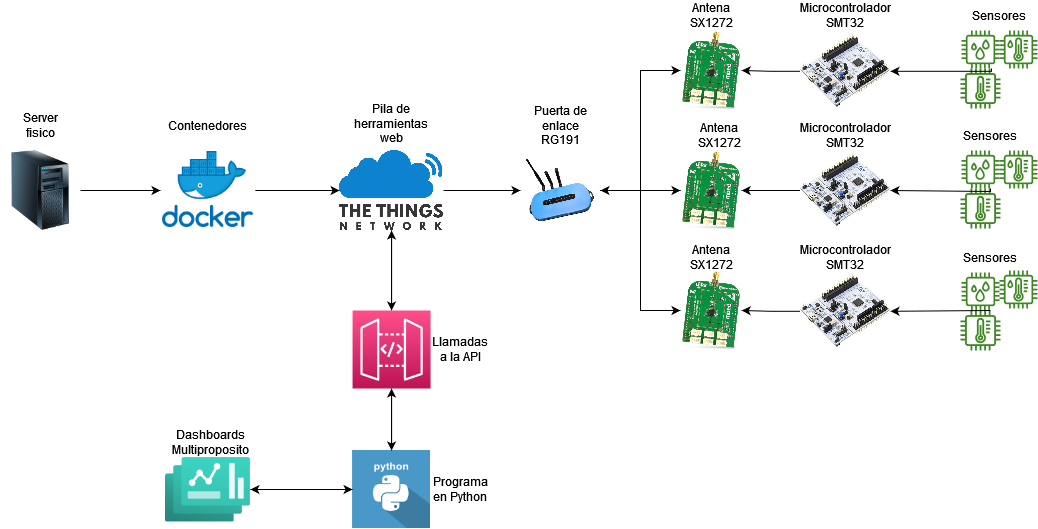
\includegraphics[width=1.0\textwidth]{imagenes/LoraWanUAGArch.png}
    \caption{Arquitectura implementada para el sistema de nodos}
    \label{fig:arquitectura-implementada}
\end{figure}

El servidor físico cuenta con una instancia de Docker para facilitar su portabilidad a otros sistemas distintos o inclusive su montaje en la nube. Dentro del contenedor se encuentra instalado The Things Stack el cual nos facilita la comunicación con múltiples puertas de enlace de tipo RG191 asi como con la administración de los nodos LoRa que funcionan atraves del microcontrolador SMT32 con su antena SX1272.
A continuación, explicare todos los pasos necesarios para la configuración y lanzamiento de un servidor.  

\section{Configuración del servidor LoRa}
 \subsection{Prerrequisitos}

Primeramente, debemos tener configurado nuestro entorno donde todo el sistema vivirá. Para este caso de uso utilizamos una distribución Debian. Para instalarlo podemos utilizar la \gls{guiadebian} proporcionada por Debian, sin embargo, tal y como explique antes. El sistema puede ser montado en cualquier sistema operativo o inclusive en la nube. 

\subsection{Instalación de Docker}

Una vez que tengamos una distribución de Linux en funcionamiento, debemos instalar Docker.Para mayor comodidad Debian ya proporciona una \href{https://docs.docker.com/engine/install/debian/}{guía de como instalar Docker} de forma sencilla en su distribución

Una vez instalado Docker podemos probar la instalación:

\begin{lstlisting}
    sudo docker run hello-world
\end{lstlisting}

Ahora, con docker instalado, podemos instalar docker-compose para facilitar la gestión de diferentes contenedores.

La forma más fácil de instalar es verificar la última versión aquí y descargar los archivos binarios más recientes usando el comando curl:

\begin{lstlisting}
   sudo curl -L https://github.com/docker/compose/releases/
   download/1.25.3/docker-compose-`uname -s`-`uname -m` 
   -o /usr/local/bin/docker-compose
\end{lstlisting}

A continuación, debemos configurar los permisos.

\begin{lstlisting}
    sudo chmod +x /usr/local/bin/docker-compose
\end{lstlisting}
    
Finalmente, solo verifique que esté funcionando

\begin{lstlisting}
    docker-compose --version
\end{lstlisting}
    

\subsection{Instalación de The Things Stack}

El siguiente paso para crear una instalación limpia es descargar los archivos de The Things Stack la cual como se explico anteriormente es la suite utilizada para el manejo de los dispositivos LoRa.
Lo primero que debemos hacer es crear una estructura de carpetas con los siguientes comandos:

\begin{lstlisting}
    mkdir the-things-stack
    mkdir config
    mkdir config/stack
\end{lstlisting}

Descargar los archivos necesarios y cámbiarle el nombre para que se pueda utilizar en Docker

\begin{lstlisting}
    curl https://www.thethingsindustries.com/docs/
    getting-started/installation/configuration/
    docker-compose-open-source.yml > docker-compose.yml
    
    curl https://www.thethingsindustries.com/docs/
    getting-started/installation/configuration/
    ttn-lw-stack-docker-open-source.yml > ttn-lw-stack-docker.yml
\end{lstlisting}

Modifique los archivos para satisfacer sus necesidades. Recuerde que puede usar archivos en el \href{https://github.com/francofonseca/lorawan_gateway}{repositorio} como ejemplo o seguir la guía de configuración oficial.

Descargar las imágenes de dockerfile

\begin{lstlisting}
    sudo docker-compose pull
\end{lstlisting}

Ahora tenemos las imágenes listas para usar.

\subsection{Configuración de certificados}

Antes de que podamos continuar configurando las imágenes de Docker, debemos asegurarnos de que podremos conectarnos a nuestro panel web sin problemas, para hacer esto, necesitamos configurar algunos certificados.

En el repositorio ya están los certificados necesarios para realizar esta tarea, en caso de que quieras crear tus certificados desde cero puedes seguir la \href{https://www.thethingsindustries.com/docs/getting-started/installation/certificates/}{guía de configuración oficial}

Para generar certificados, necesitaremos herramientas cfssl. Esta herramienta está construida con el lenguaje de programación Go, por lo que, para empezar, debemos descargar la \href{https://go.dev/dl/}{versión más reciente de la página web de Go}.

Antes de que podamos continuar configurando las imágenes de nuestra ventana acoplable, debemos asegurarnos de que podremos conectarnos a nuestro tablero sin problemas, para hacer esto, necesitamos configurar algunos certificados.

En el repositorio ya están los certificados necesarios para realizar esta tarea, en caso de que quieras crear tus certificados desde cero puedes seguir la guía de configuración oficial

Despues:

\begin{lstlisting}
    #Descomprimir Go
    tar -xzf go1.19.4.linux-amd64.tar.gz

    #Mover GO a la carpeta local
    sudo mv go /usr/local/

    #Configurar GOROOT env var
    export GOROOT=/usr/local/go

    #Verificar instalacion
    go --version
\end{lstlisting}


Ahora, con Go ejecutándose, necesitamos descargar las herramientas de cfssl. Podemos hacerlo desde el repositorio de cfssl.

\begin{lstlisting}
    git clone https://github.com/cloudflare/cfssl.git

    #Moverse dentro de la carpeta generada
    cd cfssl

    #Construir el repositorio
    make
\end{lstlisting}

Una vez que los pasos sean exitosos, se creará una carpeta bin, agregue esta ruta a la variable de entorno PATH como esta

\begin{lstlisting}
    export PATH="/home/uaguser/Downloads/cfssl/bin:$PATH"
\end{lstlisting}

Ahora necesitamos crear el archivo de certificado llamado ca.json con el siguiente contenido

\begin{lstlisting}
    {
        "names": [
            {
                "C": "NL", 
                "ST": "Noord-Holland", 
                "L": "Amsterdam", 
                "O": "The Things Demo"
            }
        ]
    }
\end{lstlisting}

Este es un ejemplo de los datos que puede modificar a su gusto siguiendo las reglas del certificado
Luego ejecute lo siguiente para generar la clave y el certificado de CA

\begin{lstlisting}
    cfssl gencert -ca ca.pem -ca-key ca-key.pem cert.json | cfssljson -bare cert
\end{lstlisting}

Ahora escriba la configuración de su certificado en cert.json

\begin{lstlisting}
    {
        "hosts": ["thethings.example.com"],
        "names": [
            {
                "C": "NL", 
                "ST": "Noord-Holland", 
                "L": "Amsterdam", 
                "O": "The Things Demo"}
        ]
    }
\end{lstlisting}

Ejecute el siguiente comando para generar la clave del servidor y el certificado

\begin{lstlisting}
    cfssl gencert -ca ca.pem -ca-key ca-key.pem 
    cert.json | cfssljson -bare cert
\end{lstlisting}


Ahora cambie el nombre de su certificado cert-key.pem a key.pem

\begin{lstlisting}
    mv cert-key.pem key.pem
\end{lstlisting}

Debian solo reconoce certificados en formato crt, por lo que es hora de convertir ambos certificados

\begin{lstlisting}
    openssl x509 -outform der -in ca.pem -out ca.crt
    openssl x509 -outform der -in cert.pem -out cert.crt
\end{lstlisting}

Copie su certificado en la carpeta de certificados, esto puede ser diferente según su distribución de Linux

\begin{lstlisting}
    sudo cp ca.crt /usr/local/share/ca-certificates/
\end{lstlisting}

Cambie los permisos de sus certificados

\begin{lstlisting}
    sudo chmod 600 /usr/local/share/ca-certificates/ca.*
    chmod 777 ca.pem 
    chmod 777 cert.pem 
    chmod 777 key.pem 
\end{lstlisting}

Actualice sus certificados

\begin{lstlisting}
    sudo update-ca-certificates
\end{lstlisting}

Su árbol de archivos ahora debería verse así, excluyendo la carpeta blob

\begin{figure}[H]
    \centering
    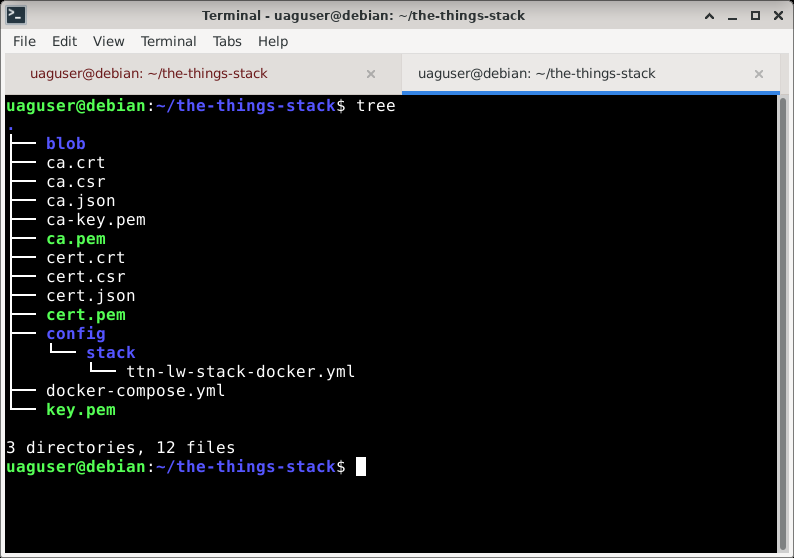
\includegraphics[width=1.0\textwidth]{imagenes/imagenes_manual/treeoffiles.png}
    \caption{Árbol de archivos}
    \label{fig:arbol-de-archivos}
\end{figure}

\subsection{Configurar LAIRD Sentrius RG191}

Ahora que configuramos los certificados, estamos listos para configurar nuestro Laird Gateway y las IP del servidor para comunicarnos.

Primero, debemos acceder a la puerta de enlace de Laird para hacerlo, consulte el \href{https://assets.lairdtech.com/home/brandworld/files/Sentrius%20RG1xx%20User%20Guide%20v2_2.pdf}{capítulo 4 de la documentación oficial} \textit{Inicie sesión en la puerta de enlace}.

Deberíamos ver algo como en la Figura \ref{fig:rg191-pagina-principal}.

\begin{figure}[H]
    \centering
    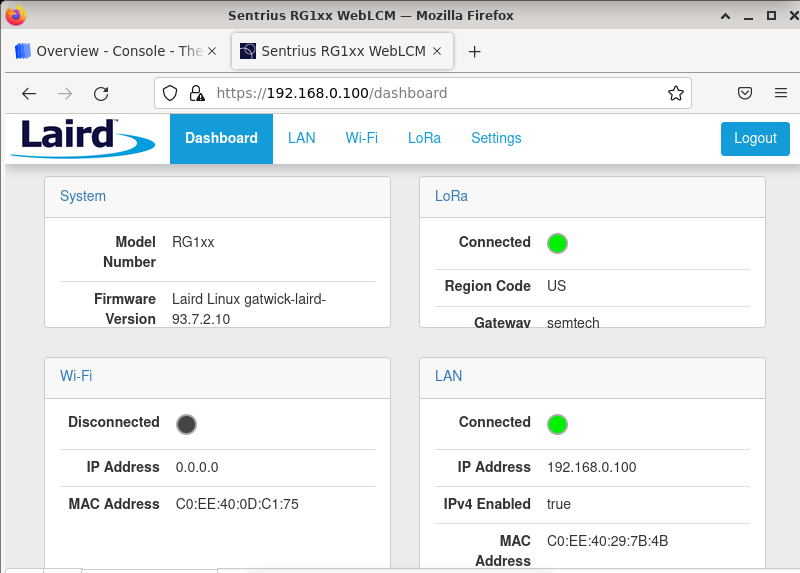
\includegraphics[width=1.0\textwidth]{imagenes/imagenes_manual/mainpagerg191.png}
    \caption{Página principal del RG191}
    \label{fig:rg191-pagina-principal}
\end{figure}

Haga clic en la pestaña LAN y rellénelo con la siguiente información y guárdelo (Figura \ref{fig:rg191-ip-estatica}).

\begin{figure}[H]
    \centering
    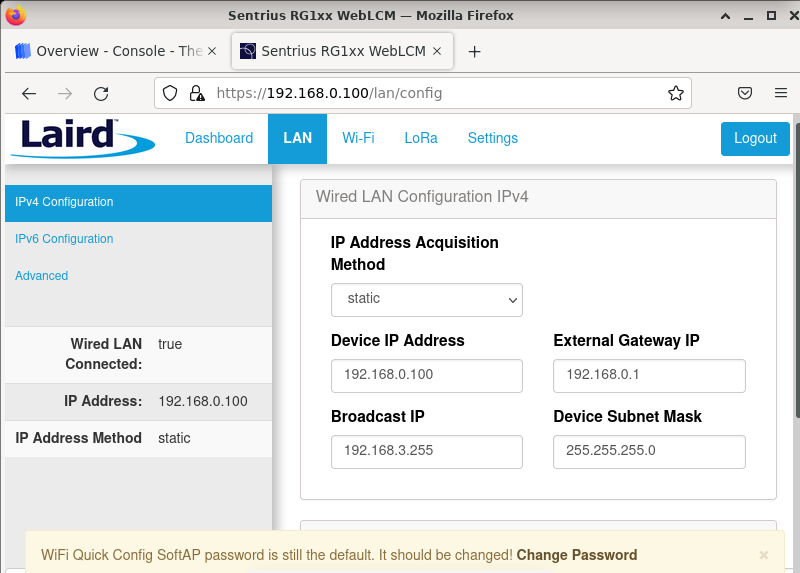
\includegraphics[width=1.0\textwidth]{imagenes/imagenes_manual/modifystatic.png}
    \caption{Modificación de IP Estática en el RG191}
    \label{fig:rg191-ip-estatica}
\end{figure}

Luego haga clic en LoRa y luego en la sección Forwarder y complete con la siguiente información y guárdela (Figura \ref{fig:rg191-lora-forwarder}).

\begin{figure}[H]
    \centering
    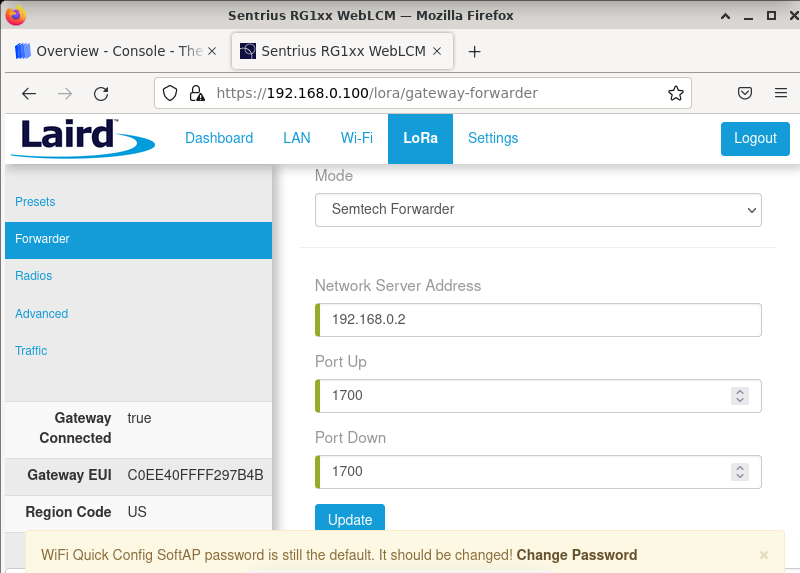
\includegraphics[width=1.0\textwidth]{imagenes/imagenes_manual/modifylora.png}
    \caption{Modificación del protocolo LoRa en el RG191}
    \label{fig:rg191-lora-forwarder}
\end{figure}

Ahora regrese al servidor, debemos verificar las interfaces disponibles para usar para comunicarnos con la puerta de enlace para hacerlo, usamos el siguiente comando

\begin{lstlisting}
    ip link show
\end{lstlisting}

En nuestro caso vamos a usar enp3s0 como interfaz para comunicarnos con la puerta de enlace para modificarla use el siguiente comando

\begin{lstlisting}
    sudo vim /etc/network/interfaces
\end{lstlisting}

Agregue la siguiente información al final del archivo y guárdelo (Figura \ref{fig:interfaz-enp3s0}).

\begin{figure}[H]
    \centering
    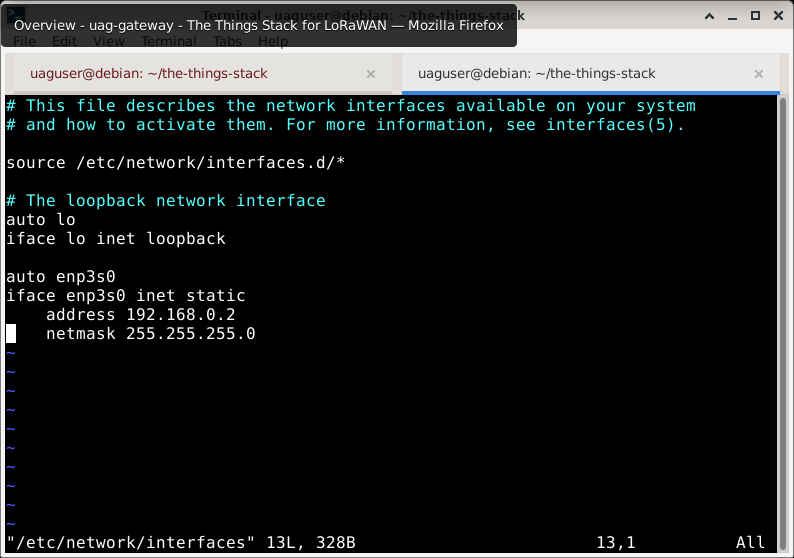
\includegraphics[width=1.0\textwidth]{imagenes/imagenes_manual/staticIP.png}
    \caption{Interfaz enp3s0}
    \label{fig:interfaz-enp3s0}
\end{figure}

Reinicie interfaces de red

\begin{lstlisting}
    sudo systemctl restart networking.service
\end{lstlisting}

Verifique que los cambios se aplicaron en la interfaz de red, en nuestro caso usamos enp3s0

\begin{lstlisting}
    ip -f inet addr show enp3s0
\end{lstlisting}

Verifique la conectividad entre Gateway y Server con el siguiente comando

\begin{lstlisting}
    ping 192.168.0.100
\end{lstlisting}

\textit{Si el ping no es exitoso, verifique nuevamente si la puerta de enlace y la interfaz están configuradas correctamente. Nota: debe perder el acceso a Internet después de este punto si usa IP privadas debido al cambio de IP de la interfaz.}

\subsection{Configurar imágenes de Docker}

Una vez que la puerta de enlace y el servidor de Laird estén configurados con direcciones IP estáticas, ahora estamos listos para configurar nuestras imágenes de Docker

Primero necesitamos migrar la base de datos.

\begin{lstlisting}
    sudo docker-compose run --rm stack is-db migrate
\end{lstlisting}

Ahora cree y administre el usuario para el panel web

\begin{lstlisting}
    sudo docker-compose run --rm stack is-db create-admin-user 
    --id admin --email yourmail@gmail.com
\end{lstlisting}

Luego habilite oauth en el panel web

\begin{lstlisting}
    sudo docker-compose run --rm stack is-db create-oauth-client     --id cli     --name "Command Line Interface"     --owner admin     --no-secret     --redirect-uri "local-callback" 
\end{lstlisting}

Cree estas dos variables de entorno para la contraseña de la consola y para la dirección del servidor

\begin{lstlisting}
    CONSOLE_SECRET="console"
    SERVER_ADDRESS="192.168.0.2"
\end{lstlisting}

Generar usuario autenticado

\begin{lstlisting}
    sudo docker-compose run --rm stack is-db create-oauth-client
    --id console --name "Console" --owner admin --secret 
    "${CONSOLE_SECRET}" --redirect-uri "${SERVER_ADDRESS}/console/
    oauth/callback" --redirect-uri "/console/oauth/callback" 
    --logout-redirect-uri "${SERVER_ADDRESS}/console"  
    --logout-redirect-uri "/console" 
\end{lstlisting}

Ahora estamos listos para ejecutar todos los contenedores.

\begin{lstlisting}
    sudo docker-compose up
\end{lstlisting}

Si todo es exitoso, deberíamos poder acceder al tablero en el siguiente enlace

\begin{lstlisting}
    https://192.168.0.2/console/
\end{lstlisting}

Ahora es el momento de pasar a configurar los dispositivos en el panale web


\section{Configurar panel web}

Una vez que accedemos al tablero desde el navegador, la primera página que deberíamos ver se verá así (Figura \ref{fig:tts-login-page}).

\begin{figure}[H]
    \centering
    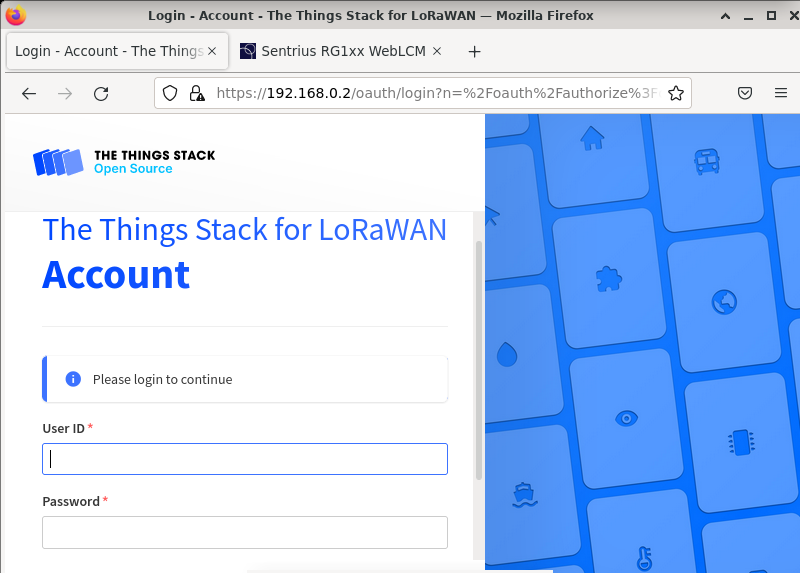
\includegraphics[width=1.0\textwidth]{imagenes/imagenes_manual/loginpage.png}
    \caption{Página principal de The Things Stack}
    \label{fig:tts-login-page}
\end{figure}

Use sus credenciales de administrador que generó previamente para iniciar sesión

\subsection{Registrar puerta de enlace}

Ahora, en la consola principal, haga clic en ir a las puertas de enlace (Figura \ref{fig:gateways-menu}).

\begin{figure}[H]
    \centering
    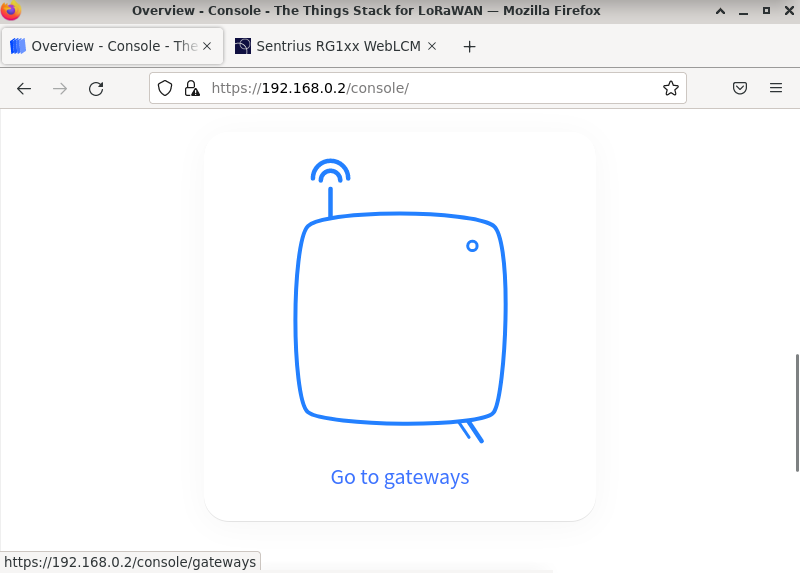
\includegraphics[width=1.0\textwidth]{imagenes/imagenes_manual/gotogateways.png}
    \caption{Icono de la sección \textit{gateways} en el panel web}
    \label{fig:gateways-menu}
\end{figure}

Ahora haga clic en registrar una puerta de enlace (Figura \ref{fig:gateways-list}).

\begin{figure}[H]
    \centering
    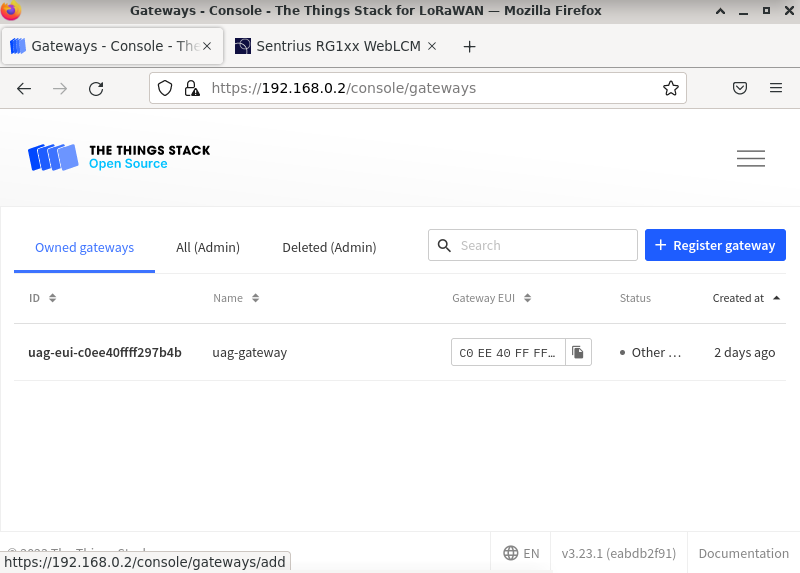
\includegraphics[width=1.0\textwidth]{imagenes/imagenes_manual/clickonregistergateway.png}
    \caption{Sección con el listado de todos los \textit{gateways} en el panel web}
    \label{fig:gateways-list}
\end{figure}

Complete los datos con su EUI correspondiente, ID de puerta de enlace y nombre de puerta de enlace, así como el plan de frecuencia (Figuras \ref{fig:gateway-register-top} y \ref{fig:gateway-register-bottom}).

\begin{figure}[H]
    \centering
    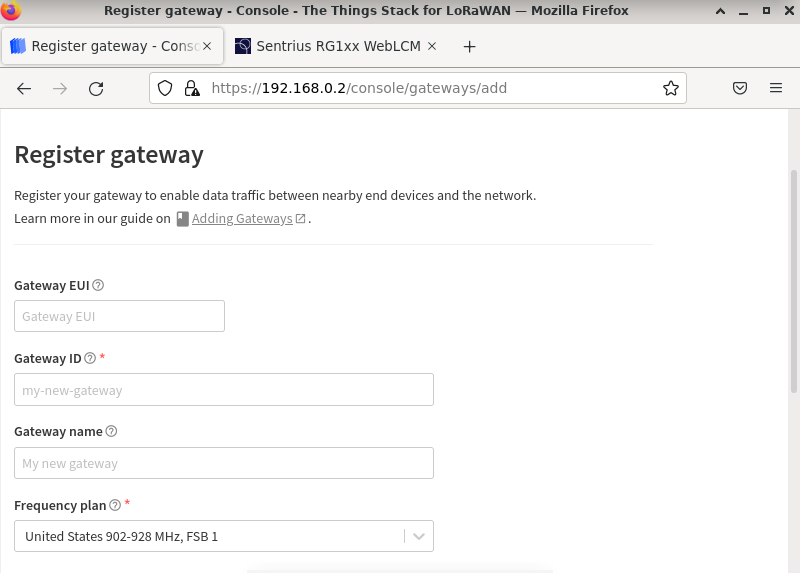
\includegraphics[width=1.0\textwidth]{imagenes/imagenes_manual/registergateway1.png}
    \caption{Sección superior de configuración para registro de un \textit{gateway}}
    \label{fig:gateway-register-top}
\end{figure}

\begin{figure}[H]
    \centering
    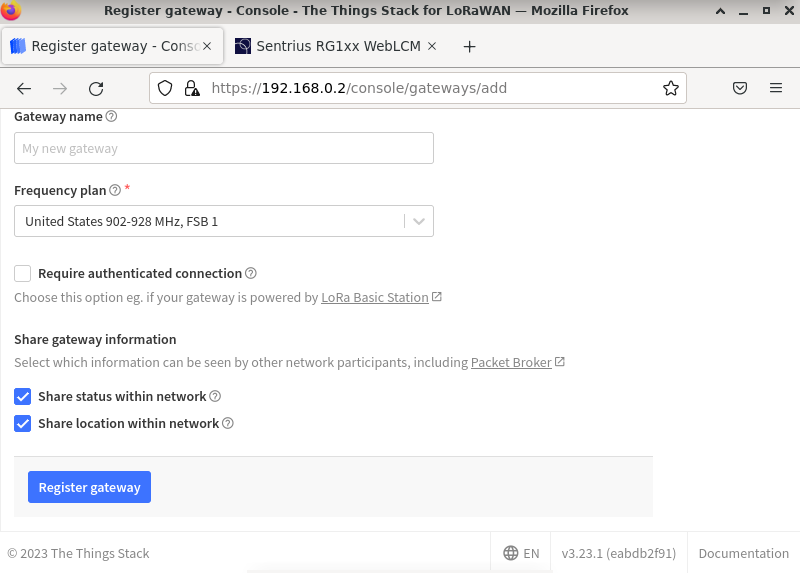
\includegraphics[width=1.0\textwidth]{imagenes/imagenes_manual/registergateway2.png}
    \caption{Sección inferior de configuración para registro de un \textit{gateway}}
    \label{fig:gateway-register-bottom}
\end{figure}

Haga clic en registrar puerta de enlace y ahora debería ver una puerta de enlace como esta (Figura \ref{fig:gateway-configured}).

\begin{figure}[H]
    \centering
    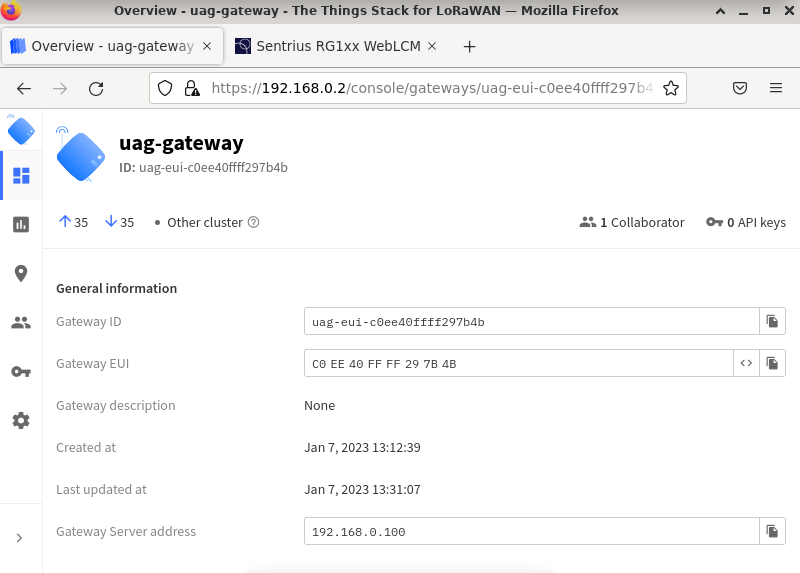
\includegraphics[width=1.0\textwidth]{imagenes/imagenes_manual/finishedgateway.png}
    \caption{Vista de un \textit{gateway} configurado}
    \label{fig:gateway-configured}
\end{figure}

También recuerde deshabilitar la conexión autenticada en caso de que quiera probar nuevos dispositivos LoRa sin credenciales (Figura \ref{fig:gateway-auth-disable}).

\begin{figure}[H]
    \centering
    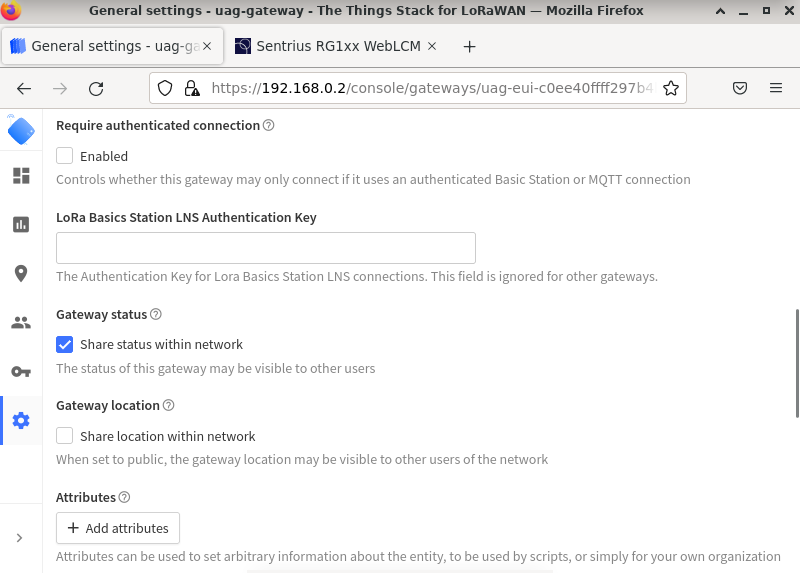
\includegraphics[width=1.0\textwidth]{imagenes/imagenes_manual/disableauth.png}
    \caption{Panel para desactivación de autenticación}
    \label{fig:gateway-auth-disable}
\end{figure}

Ahora puede ver que todo fue exitoso una vez que comenzó a recibir datos en vivo (Figura \ref{fig:gateway-traffic}) de su puerta de enlace (esto puede demorar hasta 1 o 2 minutos dependiendo de la latencia).

\begin{figure}[H]
    \centering
    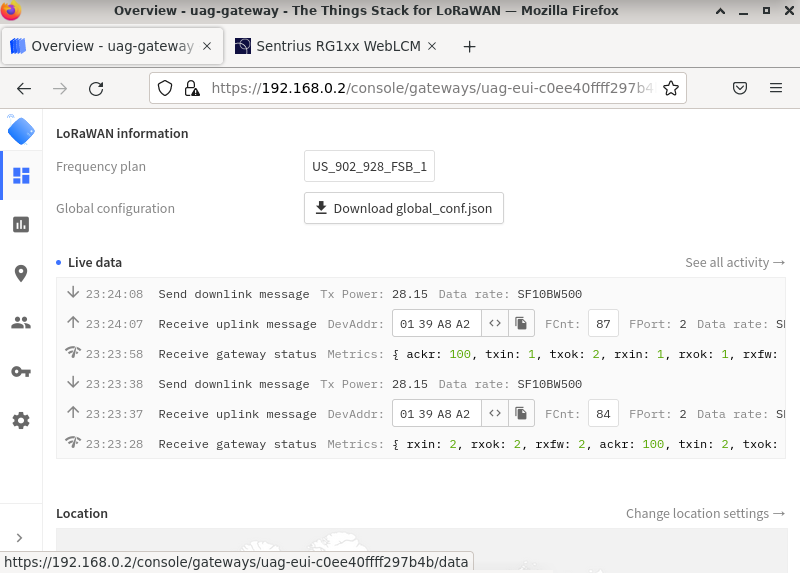
\includegraphics[width=1.0\textwidth]{imagenes/imagenes_manual/trafficgateway.png}
    \caption{Trafico de la red interceptado en el \textit{gateway}}
    \label{fig:gateway-traffic}
\end{figure}

\textit{Recuerda que si aún no tienes dispositivos solo verás mensajes administrativos}

\subsection{Crear una aplicación}

Ahora estamos listos para configurar una aplicación, esto se usa para encapsular todos los dispositivos en un solo punto y tomar información. Para hacerlo, regrese a la página principal de la consola y haga clic en ir a aplicaciones (Figura \ref{fig:applications-menu}).

\begin{figure}[H]
    \centering
    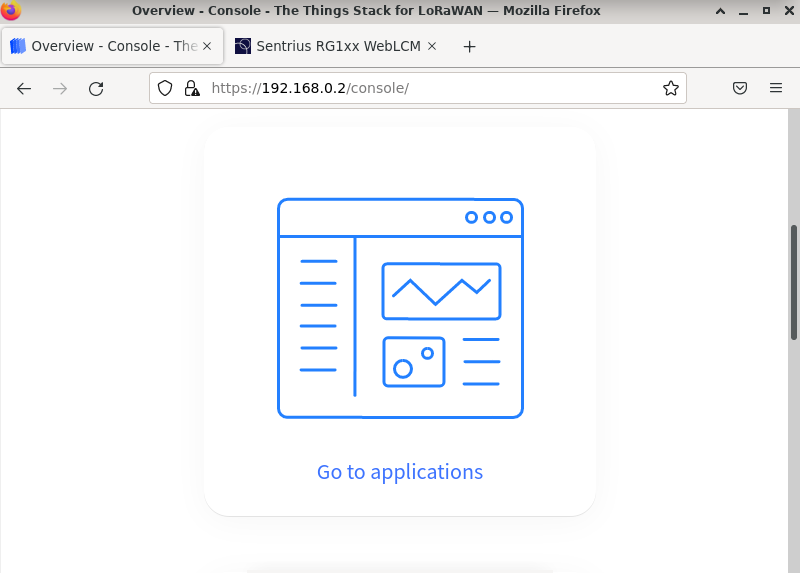
\includegraphics[width=1.0\textwidth]{imagenes/imagenes_manual/gotoapps.png}
    \caption{Icono de la sección \textit{applications} en el panel web}
    \label{fig:applications-menu}
\end{figure}

Haga clic en crear una aplicación (Figura \ref{fig:applications-list}).

\begin{figure}[H]
    \centering
    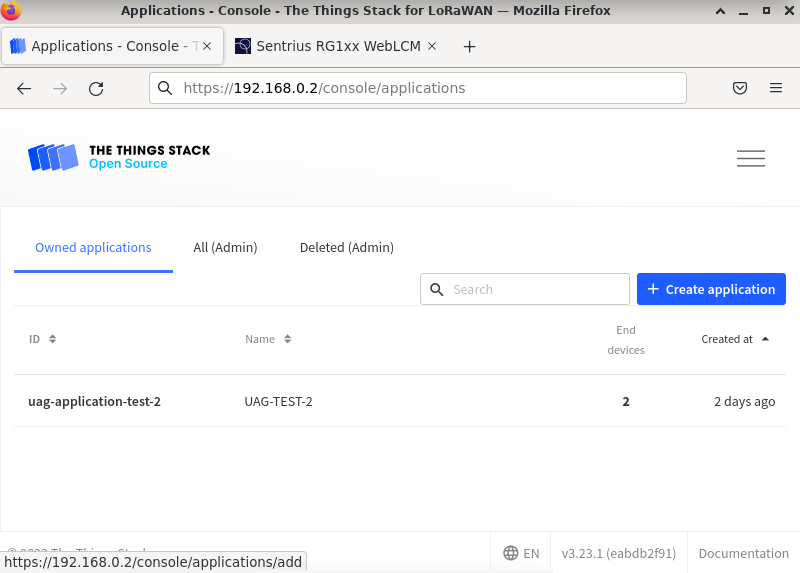
\includegraphics[width=1.0\textwidth]{imagenes/imagenes_manual/createapp.png}
    \caption{Sección con el listado de todos los \textit{applications} en el panel web}
    \label{fig:applications-list}
\end{figure}

Rellénelo con información básica sobre su aplicación y asígnele una identificación única (Figura \ref{fig:application-config}).

\begin{figure}[H]
    \centering
    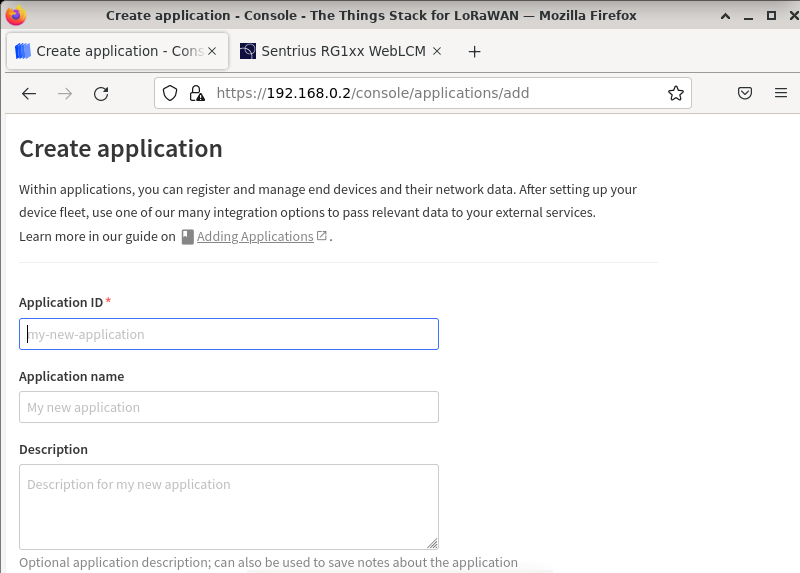
\includegraphics[width=1.0\textwidth]{imagenes/imagenes_manual/createapp2.png}
    \caption{Sección de configuración para registro de un \textit{application}}
    \label{fig:application-config}
\end{figure}

Una vez hecho esto, será redirigido a la página de su aplicación (Figura \ref{fig:application-view}).

\begin{figure}[H]
    \centering
    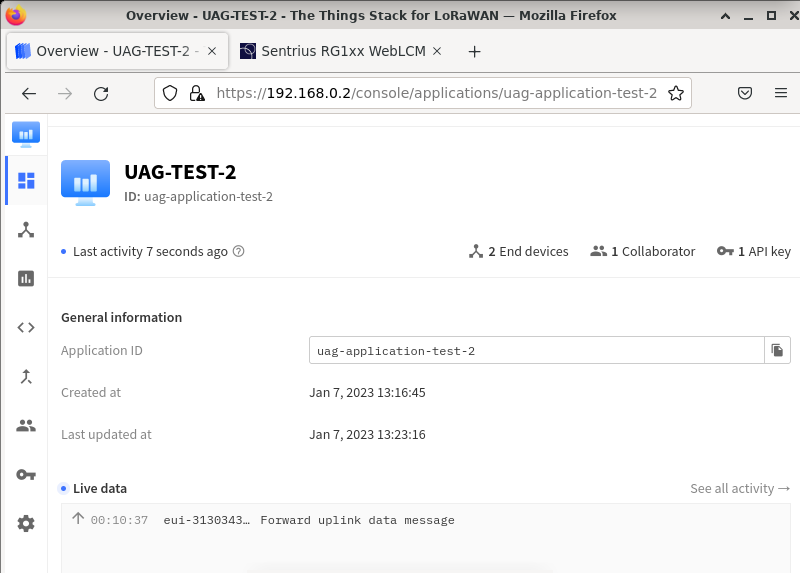
\includegraphics[width=1.0\textwidth]{imagenes/imagenes_manual/apppage.png}
    \caption{Vista de una \textit{application} configurada}
    \label{fig:application-view}
\end{figure}

\subsection{Registrar un nuevo dispositivo}

Ahora necesitamos agregar algunos nodos o dispositivos a nuestra aplicación para comenzar a capturar datos. Haga clic en Dispositivos finales en la columna izquierda de su aplicación y será redirigido a algo como esto (Figura \ref{fig:device-section}).

\begin{figure}[H]
    \centering
    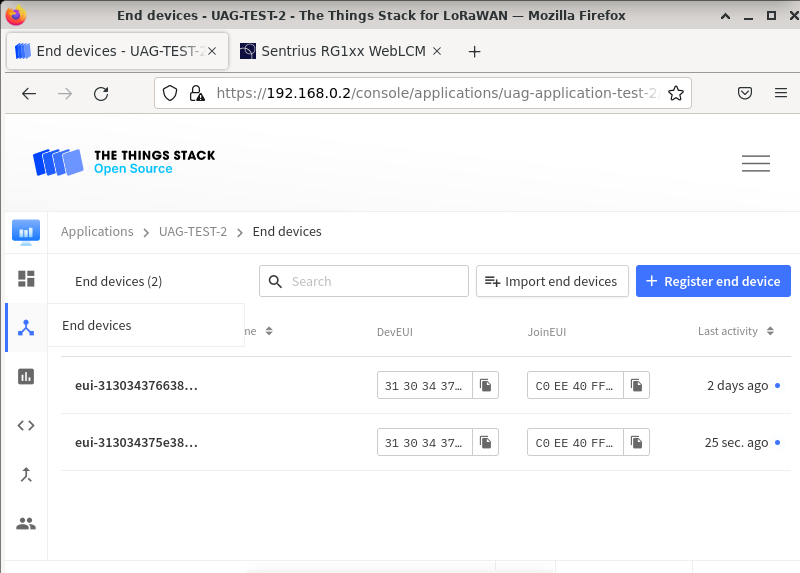
\includegraphics[width=1.0\textwidth]{imagenes/imagenes_manual/enddev.png}
    \caption{Sección superior de configuración para registro de un \textit{device}}
    \label{fig:device-section}
\end{figure}

Haga clic en Registrar dispositivo final y será redirigido nuevamente al formulario de registro de dispositivo final, haga clic en ingresar manualmente los detalles del dispositivo final (Figura \ref{fig:device-register}).

\begin{figure}[H]
    \centering
    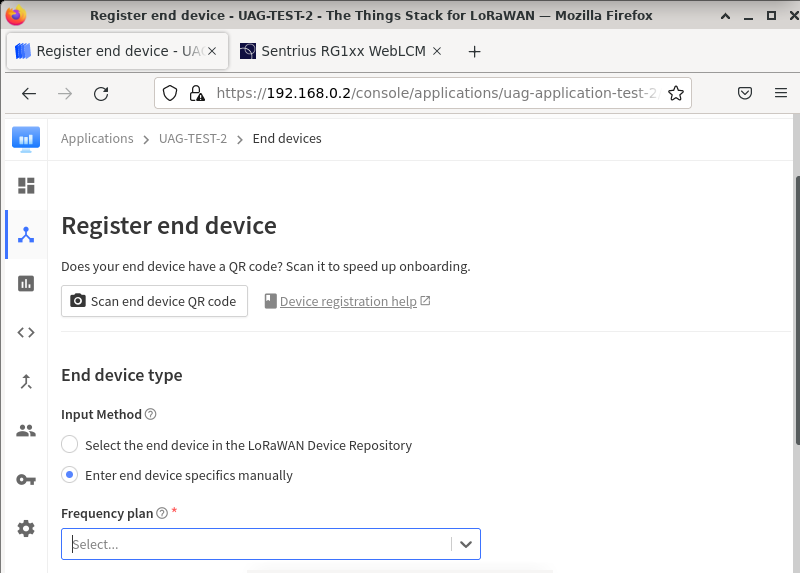
\includegraphics[width=1.0\textwidth]{imagenes/imagenes_manual/registerenddev.png}
    \caption{Sección superior de configuración para registro de un \textit{device}}
    \label{fig:device-register}
\end{figure}

Seleccione el plan de frecuencia adecuado y la especificación LoRaWAN (Figura \ref{fig:device-frequency}).

\begin{figure}[H]
    \centering
    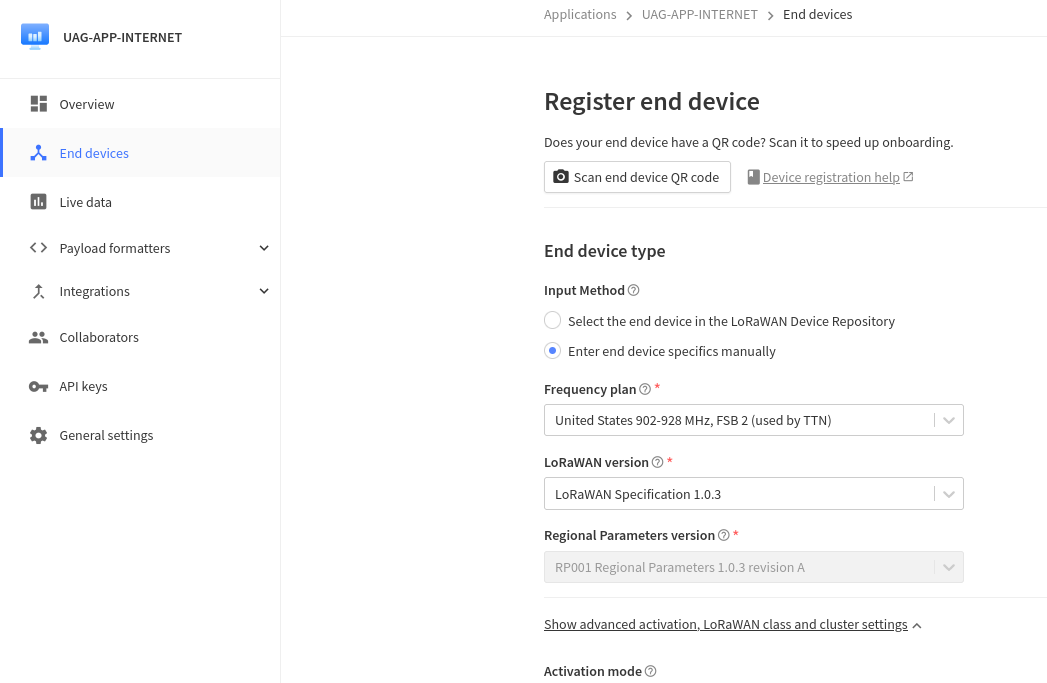
\includegraphics[width=1.0\textwidth]{imagenes/imagenes_manual/registerenddev2.png}
    \caption{Sección de frecuencia de configuración para registro de un \textit{device}}
    \label{fig:device-frequency}
\end{figure}

Debido a errores en la implementación, recomendamos el uso de 1.0.3.

Use activación de aire OTAA y clase A únicamente, también mantenga la configuración predeterminada de MAC (Figura \ref{fig:device-otaa}).

\begin{figure}[H]
    \centering
    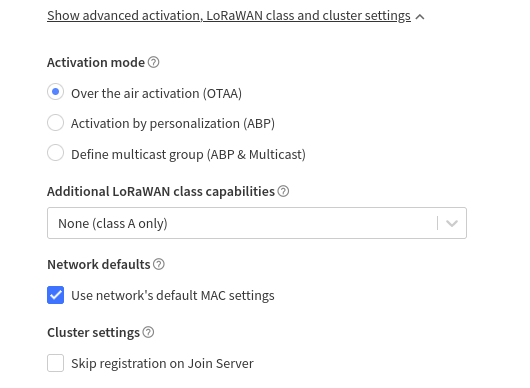
\includegraphics[width=1.0\textwidth]{imagenes/imagenes_manual/registerenddev3.png}
    \caption{Sección media de configuración para registro de un \textit{device}}
    \label{fig:device-otaa}
\end{figure}

Agregue JoinEUI, este es básicamente el mismo EUI que viene con su puerta de enlace que se usa para comunicarse en ambos sentidos (Figura \ref{fig:device-join-eui}).

\begin{figure}[H]
    \centering
    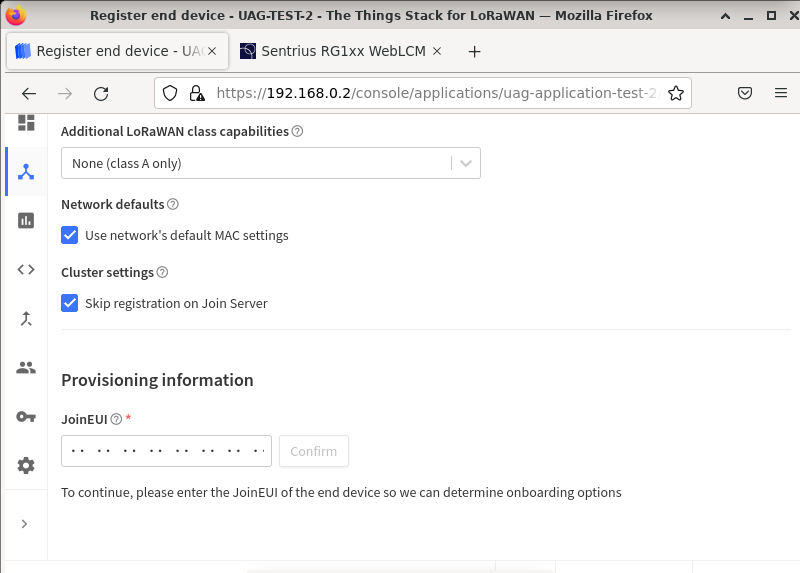
\includegraphics[width=1.0\textwidth]{imagenes/imagenes_manual/registerenddev4.png}
    \caption{Sección inferior de configuración para registro de un \textit{device}}
    \label{fig:device-join-eui}
\end{figure}

Haga clic en confirmar y ahora podrá ver el dispositivo en su aplicación, así como acceder a él (Figura \ref{fig:device-configured}).

\begin{figure}[H]
    \centering
    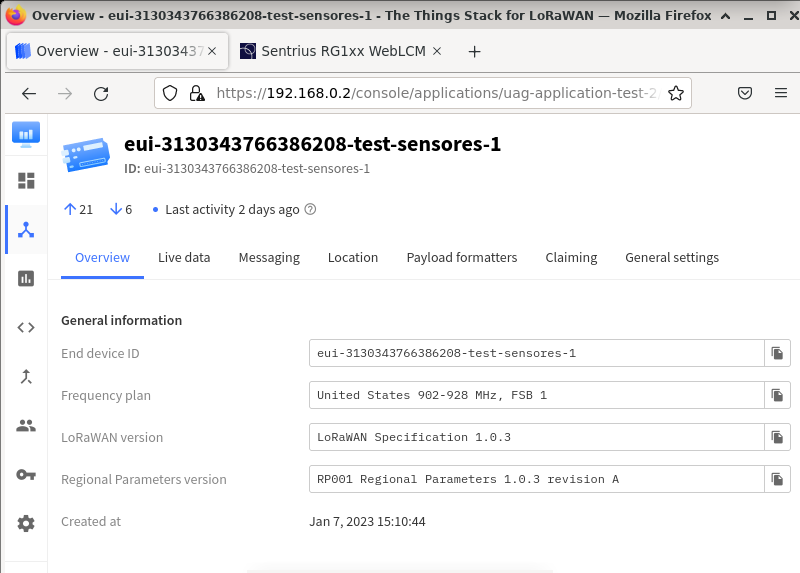
\includegraphics[width=1.0\textwidth]{imagenes/imagenes_manual/deviceexample.png}
    \caption{Vista de un \textit{device} configurado}
    \label{fig:device-configured}
\end{figure}

Ahora todo está configurado, Conecte su dispositivo a la corriente y comenzará a recibir datos en poco tiempo justo como en la siguiente imagen (Figura \ref{fig:device-live-data}).

\begin{figure}[H]
    \centering
    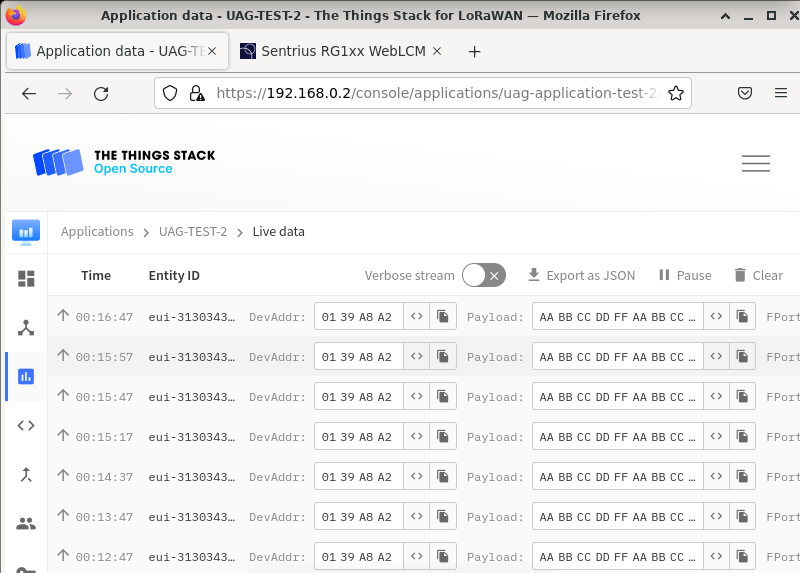
\includegraphics[width=1.0\textwidth]{imagenes/imagenes_manual/livedatafromnode.png}
    \caption{Vista de un \textit{device} configurado}
    \label{fig:device-live-data}
\end{figure}

\subsection{Leer información usando Linux}

Una vez lanzadas todas las herramientas explicadas en los capítulos anteriores podemos notar que empezamos a recibir información a través del panel web (Figura \ref{fig:device-live-data}) sin embargo podemos extender su funcionalidad leyendo la información utilizando la terminal de comandos. Gracias a esto, podemos tomar generar capas extra de funcionalidad.

La lectura de información del panel web se hace a través de su interfaz de programación de aplicaciones, utilizando el comando curl:

\begin{lstlisting}
    curl --cacert cert.pem \
    "https://192.168.0.2/api/v3/events" \
    -X POST -H "Authorization: Bearer $API_KEY" \
    -H "Accept: text/event-stream" \
    -H 'Connection: keep-alive' \
    --data-raw $'{"identifiers":[{"application_ids":
    {"application_id":"uag-application-test-2"}}]}\n'
\end{lstlisting}

El comando se compone de múltiples opciones.

La primer linea llama el comando curl asi como su certificado \textit{cert.pem} (Generado previamente para el lanzamiento del panel web)

La segunda linea utiliza la dirección IP del panel web con la ruta \textit{/api/v3/events}

La tercera linea habla del método de llamada \textit{POST} asi como del uso de la variable \textit{API\_KEY} la cual es generada a través del panel web.

La cuarta linea describe el método de comunicación el cual usara un flujo de datos por eventos basados en texto

La quinta linea especifica el mantener la conexión viva y funcionando mientras sigamos necesitando datos.

Por ultimo las dos últimas líneas describen los datos que obtendremos de la interfaz, los cuales son datos de la aplicación \textit{uag-application-test-2}, estos pueden ser modificados consultando la documentación oficial de la interfaz. 

Una vez obteniendo los datos obtendremos una cadena de texto tipo JSON, en la cual podremos encontrar múltiples datos relacionados a la llamada entre servidor y nodo, para nuestros propósitos el mas importante es el llamado payload. Este son los datos encriptados del nodo, los cuales están codificados en base64 para su mayor seguridad. Podemos desencriptarlos con alguna herramienta web o utilizando el programa en Python que se vera en la siguiente sección.

\subsection{Leer información usando código en Python}

Una capa extra añadida en nuestra investigación es el uso de un programa automatizado para la recopilación y administración de datos, como prerrequisito necesitamos apoyarnos del comando de Linux que vimos en la sección anterior y enviar los datos a un archivo con el uso del redireccionamiento de datos o con el operador doble mayor que. \[ \gg \]

Una vez que dejemos corriendo este comando empezaremos a recabar datos en un archivo de manera continua y estaremos listos para correr nuestro programa en Python. El cual nos ayuda a separar la información y agregar personalización dependiendo de los requisitos de los usuarios.

El código es el siguiente:


\begin{lstlisting}
#!/usr/bin/env python 

"""
This script is used to retrieve last data from server API and send it
to a desired dashboard.

Usage: python middleware.py
"""
import requests
import json
import base64

#INDEXES MEANING
DEVICE_ID   = 0
PAYLOAD     = 1
# URL Where are you storing logs of the server
# Feel free to change to suit your needs
SERVER_LOGS_PATH='/tmp/logs_pako.txt'

# External dashboard URL and headers
# Feel free to modify it to suit your needs
dashboard_url = "https://sistema-incendios-uag.up.railway.app\
/api/nodes-data"
dashboard_headers = {
    'Accept'        : 'application/json',
    #API_KEY
    'Authorization' : 'Bearer 7|yvXruJRQtoWNqsNZYQQdrmLqNj69mIg4ej06RkFn', 
    'Content-Type'  : 'application/json'
}

def decrypt_data(string):
    """
    Function to decrypt any data in base64 to binary
    """
    decode_payload = base64.b64decode(string.encode('ascii'))
    return decode_payload.hex()

def call_node_data():
    """
    Read the logs from the watcher
    """
    with open(SERVER_LOGS_PATH, 'r') as f:
        last_line = f.readlines()[-3]
    response = json.loads(last_line)
    #Get the payload
    return [response['result']['identifiers'][0]['device_ids']['device_id'],response['result']['data']['uplink_message']['frm_payload']]

def format_payload(payload, device_id):
    """
    Here we can format the payload to our needs
    """
    #IMPORTANT for this example we are sending all the PAYLOAD as
    #TEMPERATURE it dependes on programmer to split data as needed
    dashboard_payload={
        "node_id": device_id,
        "temperature" : payload,
        # "gas": 69,
        # "humidity": 666,
        # "fire": 420 
    }
    return dashboard_payload

def submit_node_data(data):
    """
    Submit node data to dashboard
    """
    response = requests.post(dashboard_url, 
    json=data, headers=dashboard_headers)
    if response.status_code != 200 | response.status_code != 201:
        print('ERROR: {}. Status code: {}'.format(
        response.reason, response.status_code))
        print('ERROR: {}'.format(response.text))
    return response

if __name__ == '__main__':
    #TODO: add persistant running with while and keep 
    #last line if changed run cycle again, if not skip until 
    #next minute or whatever time we want
    
    # Get data from nodes
    response = call_node_data()
    # Decrypt payload
    raw_payload = decrypt_data(response[PAYLOAD])
    # Format payload
    dashboard_payload = format_payload(raw_payload, 
    response[DEVICE_ID])
    # Print message to be sent
    print(dashboard_payload)
    # Send the message to dashboard
    submit_node_data(dashboard_payload)
\end{lstlisting}

El programa se compone de cuatro funciones principales.

La primera función \textit{call\_node\_data} hace el llamado del archivo donde guardamos los datos, leyendo las ultimas líneas y transformándolas en un objeto JSON para extraer los datos del nodo.

La segunda función \textit{decrypt\_data} nos ayuda a desencriptar los datos en base64 de forma automática, obteniendo una trama legible en texto plano.

Mas adelante la tercera función \textit{dashboard\_payload} nos ayuda a formar una nueva trama la cual será enviada por la función \textit{submit\_node\_data}


\subsection{Problemas comunes encontrados y sus soluciones}

P: ¿Qué debo hacer para instalar Debian sin internet en el servidor?

R: Como el servidor está aislado sin una interfaz Wi-Fi, recomendamos descargar una imagen de \href{https://www.debian.org/CD/http-ftp/}{CD/DVD}, que tiene más memoria, pero la ventaja es que viene con muchas herramientas preconstruidas instaladas como un entorno de escritorio.

P: No puedo conectarme a la URL de API, ¿qué puedo hacer?

R: A partir del 11 de enero de 2023, existe un problema conocido con respecto al archivo ttn, agregue este código a continuación en console.ui Verifique el archivo del repositorio como referencia

\begin{lstlisting}
    dcs:
      base-url: "https://192.168.0.2/api/v3"
\end{lstlisting}

P: Al instalar Go hay un error con una variable llamada GOPATH que no me deja continuar, ¿qué puedo hacer?

R: Si se configura GOPATH, se producirá un error al eliminar esta variable.

\begin{lstlisting}
    unset GOPATH
\end{lstlisting}

P: Al instalar Go, hay un error con respecto al comando make.

R: En caso de que no tenga el comando make, instale las herramientas esenciales en Debian, el comando es

\begin{lstlisting}
    sudo apt-get install build-essential
\end{lstlisting}

P: No puedo iniciar el tablero usando Redactar debido a un puerto de error

R: A veces, otros servicios toman algunos puertos necesarios para que el tablero funcione para verificar qué servicios están actualmente tomando puertos y ejecutándose, use el siguiente comando

\begin{lstlisting}
    sudo ss -nlpt
\end{lstlisting}

En nuestro caso, apache2 estaba tomando el puerto 80, por lo que necesitamos detenerlo.

\begin{lstlisting}
    sudo service apache2 stop
\end{lstlisting}

P: Completé la información de la puerta de enlace pero no se registró

R: A veces, la información de la puerta de enlace no se registra como se esperaba y tenemos que modificarla manualmente. Para hacerlo, vaya a la configuración y modifique el campo de dirección del servidor de la puerta de enlace (Figura \ref{fig:gateway-ip-settings}).

\begin{figure}[H]
    \centering
    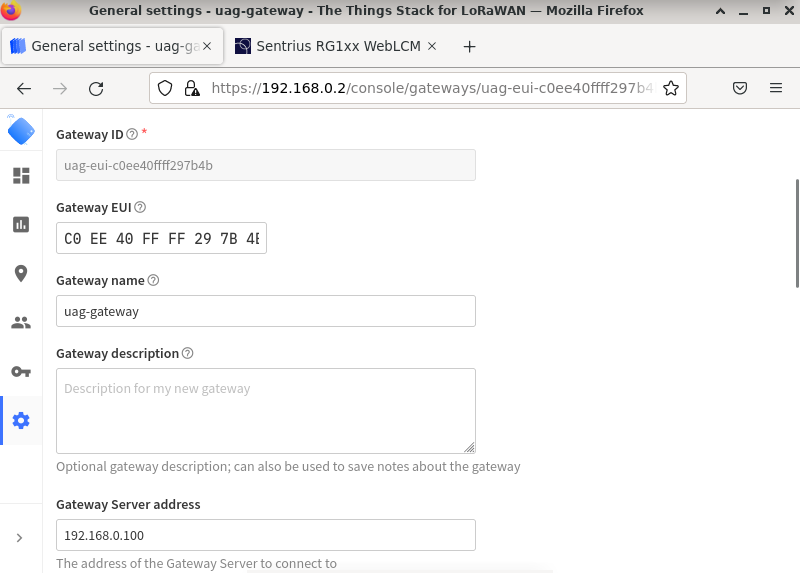
\includegraphics[width=1.0\textwidth]{imagenes/imagenes_manual/changestaticIP.png}
    \caption{Vista de configuración para la IP de un \textit{gateway}}
    \label{fig:gateway-ip-settings}
\end{figure}

P: No puedo entender que la carga útil parece estar encriptada

R: Puede deshabilitar los formateadores de la carga útil para ver los datos sin formato en caso de que quiera probar. Vaya a formateadores de carga útil en su dispositivo y seleccione Ninguno (Figura \ref{fig:payload-format-view}).

\begin{figure}[H]
    \centering
    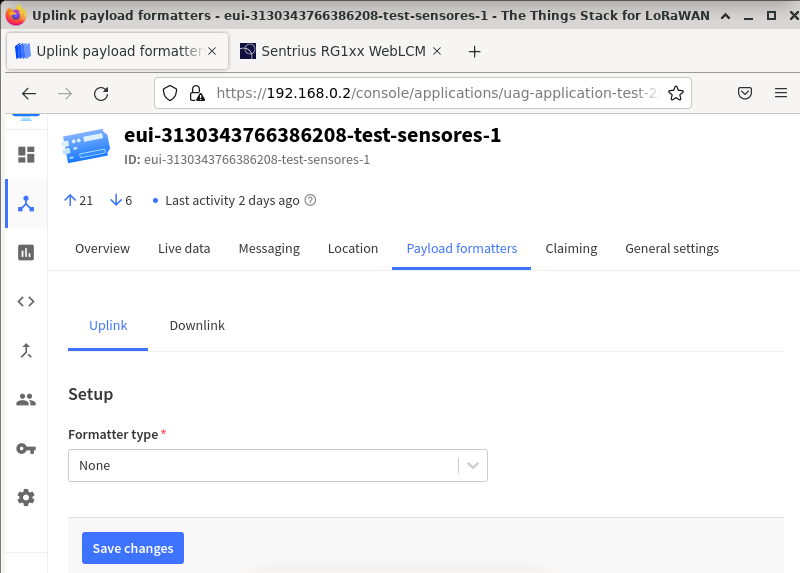
\includegraphics[width=1.0\textwidth]{imagenes/imagenes_manual/disablepayloadformatters.png}
    \caption{Vista para el formato de los paquetes}
    \label{fig:payload-format-view}
\end{figure}

Guardar los cambios

P: La aplicación no me permite registrar un dispositivo porque ya está en uso

R: Cambie el EUI de su dispositivo y cambie la ID del dispositivo una vez que se registre en la aplicación

P: No puedo revisar los mensajes de datos en vivo en el tablero

R: A veces, este problema se debe a que la puerta de enlace no puede comunicarse con los nodos, verifique dos veces los EUI de la puerta de enlace y los dispositivos e intente volver a conectarse con la puerta de enlace usando el comando ping a la IP.